\section{Epilepsia}
La epilepsia es uno de los primeros trastornos documentados en la historia de la neurología. Su aparición se remonta a más de 3.000 años atrás, siendo mencionada por primera vez en la antigua Babilonia. No obstante, fue en el año 400 a.C. cuando Hipócrates señaló que la epilepsia era un trastorno cerebral. La palabra ``epilepsia'' proviene del griego y significa ``ataque''. A lo largo de la historia, el peculiar comportamiento provocado por ciertos tipos de crisis convulsivas ha dado lugar a numerosas supersticiones y prejuicios \cite{wyllie2006treatment}.

Una crisis epiléptica consiste en una alteración brusca y transitoria ocasionada por una actividad anormal de las neuronas, manifestándose a través de sensaciones, emociones y comportamientos extraños, espasmos musculares y pérdida de conciencia. La epilepsia implica una predisposición a experimentar crisis epilépticas recurrentes, siendo diagnosticada cuando una persona ha experimentado dos o más de estas crisis. Las crisis epilépticas se dividen en dos tipos principales: crisis generalizadas y crisis parciales o focales. En las crisis generalizadas, la descarga epiléptica afecta simultáneamente a toda la superficie del cerebro, mientras que en las crisis parciales o focales, la descarga epiléptica se origina en una parte específica del cerebro \cite{garcia2011feen}.

\subsection{Tipos de epilepsia}
Existen varios tipos de epilepsia, que se clasifican en función del tipo de crisis que experimenta una persona. Algunos tipos comunes de epilepsia son:
\begin{itemize}
    \item Epilepsia focal: Las crisis focales, también llamadas crisis parciales, se originan en una parte específica del cerebro. Estas crisis pueden hacer que la persona experimente sensaciones o movimientos en un lado del cuerpo.
    \item Epilepsia generalizada: Las crisis generalizadas afectan a ambos lados del cerebro. Estas crisis pueden hacer que la persona pierda el conocimiento, caiga al suelo y experimente espasmos musculares o convulsiones.
    \item Epilepsia de ausencia: Las crisis de ausencia, también llamadas crisis de pequeño mal, hacen que la persona se quede con la mirada perdida y pierda temporalmente la conciencia de lo que le rodea.
    \item Epilepsia tónico-clónica: Las crisis tónico-clónicas, también llamadas crisis de gran mal, son el tipo de crisis más conocido. Implican pérdida de conocimiento, caída al suelo y movimientos espasmódicos repetitivos del cuerpo.
    \item Epilepsia mioclónica juvenil: Este tipo de epilepsia suele comenzar en la adolescencia. Se caracteriza por breves sacudidas o espasmos musculares, especialmente por la mañana después de despertarse. 
\end{itemize}

\begin{figure}[t]
    \centering
    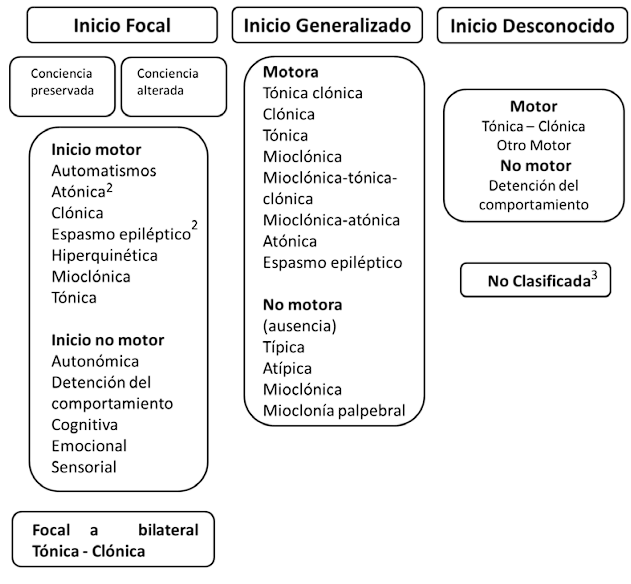
\includegraphics[width=0.5\textwidth]{figuras/6 Ictal_class.png}
    \caption{Clasificación Operacional Extendida de los tipos de crisis \cite{Clasificacion_ictal_imag}.}
    \label{fig:clasificacion_ictal_ref_imag}
\end{figure}

La Liga Internacional contra la Epilepsia (ILAE) ha introducido una categorización operativa actualizada de los tipos de crisis, mostradas en la Figura~\ref{fig:clasificacion_ictal_ref_imag}. La clasificación general incluye las crisis generalizadas, las crisis focales, también denominadas crisis de inicio parcial, y las crisis de origen desconocido. Estos tipos de crisis se clasifican a su vez en subcategorías basadas en síntomas motores y no motores. Además, en el caso de las crisis focales, existe otra distinción entre las que cursan con consciencia normal y las que presentan un nivel de consciencia alterado \cite{Clasificacion_ictal_imag}. 

\section{Señales bioeléctricas}
Las señales bioeléctricas son señales eléctricas producidas en los seres vivos que pueden medirse y controlarse continuamente. Estas señales suelen ser generadas por sistemas especializados de tejidos, órganos o células, como el sistema nervioso. Las señales bioeléctricas tienen características únicas que las hacen útiles en una amplia gama de aplicaciones, como la cardiología, la neurología y la ingeniería biomédica \cite{señales_unam}.

\section{Señales electroencefalográficas}
La electroencefalografía (EEG) es una prueba de diagnóstico neurofisiológico que consiste en la medición de la actividad eléctrica cerebral en estado de reposo, vigilia o sueño, y durante diversas activaciones. En general, la electroencefalografía se utiliza para el análisis de la actividad eléctrica cerebral en humanos con el fin de obtener información para una inspección exhaustiva de la funcionalidad cerebral, ayudando a la detección y prevención de enfermedades y trastornos. Estas ondas cerebrales se conocen como señales electroencefalográficas (señales EEG), que proporcionan información indirecta relacionada con las funciones cerebrales, incluidas, entre otras, las tareas mentales, las acciones motoras y las expresiones faciales \cite{manipula_arm_eeg}.

\subsection{Ritmos y formas de onda del EEG}
A continuación se resumen brevemente las características de los ritmos y formas de onda más frecuentes, que también se puede observar en la Figura~\ref{fig:eeg_ritmo_cerebral}. 
Las señales EEG registradas tienen, en amplitudes que oscilan entre unos pocos micro-voltios y aproximadamente 100 uV y un contenido frecuencial que oscila entre 0.5 y 30-40 Hz. Los ritmos electroencefálicos, también denominados ritmos de fondo, se clasifican convencionalmente en cinco bandas de frecuencia diferentes. La interpretación de estas bandas en términos de ``normal'' o ``anormal'' es relativa y depende de la edad y el estado mental del sujeto. Por ejemplo, el EEG de un recién nacido es drásticamente diferente del de un adulto y tiene, en general, un contenido de frecuencias considerablemente más alto.
\begin{itemize}
    \item Ritmo delta, <4 Hz. El ritmo delta suele aparecer durante el sueño durante profundo y tiene una gran amplitud. El adulto despierto y normal, pero es indicativo, por ejemplo, de daño cerebral o enfermedad cerebral (encefalopatía).
    \item Ritmo theta, 4-7 Hz. El ritmo theta se produce durante la somnolencia y en ciertas fases del sueño.
    \item Ritmo alfa, 8-13 Hz. Este ritmo es más prominente en sujetos normales que están relajados y despiertos con los ojos cerrados; la actividad se suprime cuando los ojos están abiertos. Cuando los ojos están abiertos. La amplitud del ritmo alfa es mayor en las regiones occipitales.
    \item Ritmo beta, 14-30 Hz. Es un ritmo rápido de baja amplitud, asociado a la activación de la corteza cerebral. Asociado a un córtex activado y que puede observarse, por ejemplo, durante ciertas fases del sueño. El ritmo beta se observa principalmente en las áreas frontal y central del cuero cabelludo.
    \item Ritmo gamma, >30 Hz. El ritmo gamma está relacionado con un estado de procesamiento activo de la información en el córtex. Utilizando un electrodo ubicado sobre el área sensoriomotora y conectado a una técnica de registro de alta sensibilidad, se puede observar el ritmo gamma.
\end{itemize}

\begin{figure}[t]
    \centering
    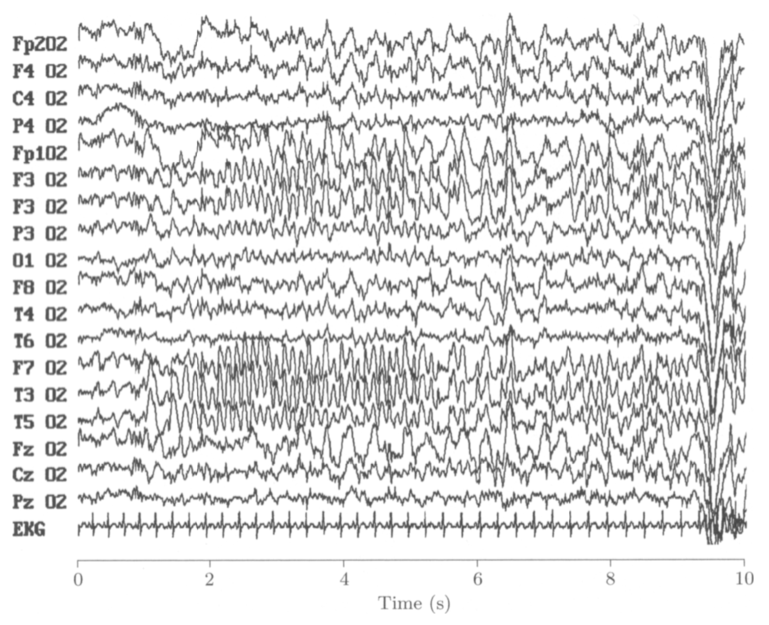
\includegraphics[width=0.5\textwidth]{figuras/7_ej_ictal_eeg.png}
    \caption{EEG multicanal que muestra el inicio de un ataque epiléptico después del primer segundo. El inicio se caracteriza por un aumento en la amplitud y un cambio en el contenido espectral. La convulsión es particularmente pronunciada en ciertos canales. Tenga en cuenta que el ECG se muestra en la parte inferior \cite{Libro_SP_cocoro_neuro_app}.}
    \label{fig:ej_ictal_multicanal_book}
\end{figure}
La mayoría de estos ritmos pueden durar varios minutos, mientras que otros sólo unos segundos. Es importante darse cuenta de que un ritmo no está presente en todo momento, una señal irregular de aspecto ``arrítmico'' \cite{Libro_SP_cocoro_neuro_app}.

\subsection{Picos y ondas agudas}
Los picos y las ondas agudas, también conocidas como SSW, son patrones distintivos en las formas de onda de EEG que tienen un patrón temporal esporádico e impredecible que indica un comportamiento neural anormal. Estos patrones se observan a menudo en pacientes que padecen epilepsia y se denominan interictales, ya que ocurren entre ataques epilépticos.

\begin{figure}[t]
    \centering
    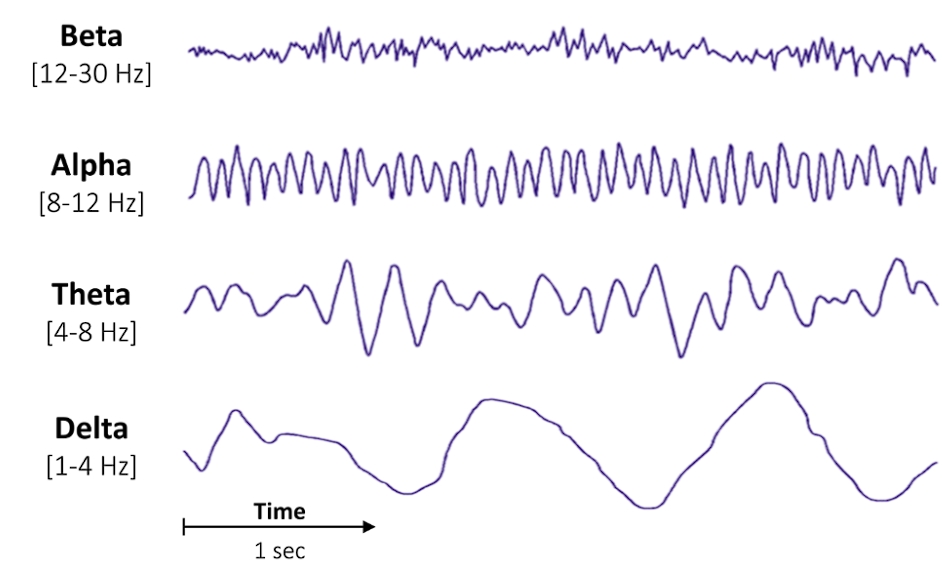
\includegraphics[width=0.5\textwidth]{figuras/8 Ritmo_cerebral_eeg.png}
    \caption{Ejemplo de ritmos cerebrales presentes en un EEG \cite{Vallat_2018}.}
    \label{fig:eeg_ritmo_cerebral}
\end{figure}

La definición de SSW es un poco ambigua, pero generalmente se caracteriza por un fuerte ascenso inicial que lo diferencia de un pico, que dura entre 20 y 70 ms. Por otro lado, SSW puede durar de 70 a 200 ms y exhibir formas de onda bifásicas y trifásicas. La morfología de SSW difiere según la ubicación del electrodo en el cuero cabelludo.

SSW puede ocurrir como eventos individuales o en series llamadas complejos de pico y onda, que consisten en un pico seguido de una onda lenta. La tasa de repetición de estos complejos puede oscilar entre menos de 3 a 6 Hz, y la tasa a menudo se asocia con diferentes interpretaciones clínicas.

Algunos artefactos EEG normales pueden parecerse a SSW, como la actividad cardíaca que puede hacerse pasar por un pico, particularmente las ondas del complejo QRS \cite{Libro_SP_cocoro_neuro_app}.

\subsection{Características de una señal EEG}
Hay una serie de características que se pueden extraer de las señales de EEG para su procesamiento. Estas funciones se pueden dividir en dos categorías principales: funciones en el dominio del tiempo y funciones en el dominio de la frecuencia.

\subsection{EEG ictal}
En el caso de una convulsión, el EEG se denomina EEG ictal y se caracteriza por un patrón inusual con un aumento repentino de la amplitud, como se muestra en la Figura~\ref{fig:ej_ictal_multicanal_book}. Además, el comienzo de una convulsión se acompaña de un cambio repentino en la amplitud. contenido de frecuencia que con frecuencia progresa a un patrón de picos y ondas. Debido a la variabilidad sustancial en el EEG ictal entre convulsiones, puede ser un desafío identificar el patrón de manera consistente, ya sea por medios manuales o automáticos \cite{Libro_SP_cocoro_neuro_app}.

\subsection{Procesamiento de señales EEG}
Las diferentes formas de onda de la señal EEG llevan información clínicamente valiosa. Una forma de onda puede representar un evento aislado, o varias formas de onda pueden constituir un patrón de señal compuesto. En ambos casos, es fundamental desarrollar métodos para detectar y cuantificar objetivamente las características de la señal para facilitar la interpretación visual. La extracción de características de señales relevantes es particularmente crucial cuando el objetivo es diseñar un sistema de clasificación de EEG. La cancelación de ruido y artefactos es otro tema importante en el procesamiento de señales de EEG y un requisito previo para el análisis de señales posterior confiable \cite{Libro_SP_cocoro_neuro_app}.

\section{Señales electromiográficas}
La electromiografía (EMG) es una herramienta de diagnóstico utilizada para analizar y registrar la actividad eléctrica producida por los músculos esqueléticos. La EMG se emplea en diversos campos de la medicina, como la neurología, la medicina deportiva, la rehabilitación y el diagnóstico. Los investigadores también utilizan la EMG para estudiar los patrones de activación muscular durante el movimiento, así como los patrones de fatiga y recuperación muscular. La EMG registra la actividad eléctrica llevada a cabo por las neuronas motoras durante las contracciones musculares y también mide la fuerza de las contracciones \cite{emg_def}. 

\section{Señales electrocardiográficas}
Un electrocardiograma (ECG) es una prueba médica común que registra la actividad eléctrica del corazón. Se utiliza para evaluar la salud y el funcionamiento del corazón, y puede ayudar a diagnosticar problemas cardíacos o monitorizar afecciones existentes. Durante un ECG, se colocan electrodos en el pecho, las extremidades y a veces en otros lugares del cuerpo, para medir y registrar la actividad eléctrica del corazón \cite{ecg_def}.

La prueba es indolora y no invasiva, lo que significa que no se introduce nada en el cuerpo. Los resultados del ECG proporcionan información sobre la frecuencia cardíaca, el ritmo cardíaco, la regularidad de los latidos y la presencia de cualquier anormalidad en la conducción eléctrica del corazón \cite{zavala2017descripcion}.


\section{Características en el dominio del tiempo}
Las características en el dominio del tiempo se basan en el análisis de la amplitud de la señal y sus cambios a lo largo del tiempo \cite{carac_time}. Algunas características comunes en el dominio del tiempo incluyen:
\begin{itemize}
    \item Media: 
    El valor promedio de la señal durante un intervalo de tiempo específico.
    \item Mediana: 
    El valor medio de la señal durante un intervalo de tiempo específico.
    \item Varianza: 
    La desviación cuadrada promedio de la señal de su valor medio.
    \item Desviación estándar: 
    La raíz cuadrada de la varianza.
    \item Asimetría: 
    Una medida de la asimetría de la distribución de la señal.
    \item Curtosis: 
    Una medida del pico de la distribución de la señal.
\end{itemize}

\section{Características en el dominio de frecuencia}
Las características en el dominio de la frecuencia se basan en el análisis del espectro de potencia de la señal. El espectro de potencia es un gráfico de la potencia de la señal en función de la frecuencia \cite{carac_freq}. Algunas características comunes en el dominio de la frecuencia incluyen:
\begin{itemize}
    \item Potencia: 
    La potencia total de la señal en una banda de frecuencia especificada.
    \item Energía: 
    La energía total de la señal en una banda de frecuencia específica.
    \item Densidad espectral: 
    La potencia de la señal por unidad de frecuencia en una banda de frecuencia especificada.
    \item Frecuencia centroide: 
    La frecuencia en la que el espectro de potencia de la señal es más alto.
    \item Propagación: 
    Una medida del ancho del espectro de potencia de la señal.
\end{itemize}

La elección de características para extraer de las señales de EEG depende de la aplicación. Por ejemplo, las funciones en el dominio del tiempo se usan a menudo para estudiar los cambios en la actividad cerebral a lo largo del tiempo, mientras que las funciones en el dominio de la frecuencia se usan a menudo para estudiar las diferentes bandas de frecuencia de la actividad cerebral \cite{al2014methods}.


\section{Propiedades de las señales deterministas y estocásticas}
Las señales deterministas son aquellas que pueden describirse mediante un conjunto de ecuaciones que definen su comportamiento en el tiempo. Las señales estocásticas, por otro lado, son aquellas que se caracterizan por fluctuaciones aleatorias.
Surge una pregunta fundamental con respecto a si el EEG debe verse como una señal determinista o estocástica. Los intentos de responder a esta pregunta pueden proporcionar información sobre los mecanismos de generación de EEG, pero también tienen implicaciones para los métodos de análisis de señales apropiados considerados. Generalmente, las características exactas de la señal EEG en términos de amplitud, duración o morfología de las ondas individuales no se pueden predecir, por lo que es bastante natural percibir la señal EEG como la realización de un proceso estocástico. Esta perspectiva cobra mayor fuerza al observar que no es posible adquirir una señal EEG ``pura'' que refleje únicamente la actividad cerebral. De hecho, siempre hay un ruido aleatorio corruptor introducido, por ejemplo, por el ruido interno en el equipo de amplificación o en el proceso de digitalización, lo que, incluso si el EEG ``puro'' tuviera propiedades deterministas, en última instancia hace que sea razonable considerar el EEG como un proceso estocástico \cite{Libro_SP_cocoro_neuro_app}.

Hay una serie de propiedades que se pueden utilizar para distinguir entre señales deterministas y estocásticas en los datos de EEG. Una propiedad es el espectro de potencia de la señal. El espectro de potencia de una señal es un gráfico de la potencia de la señal en función de la frecuencia. Las señales deterministas suelen tener un espectro de potencia que se caracteriza por picos pronunciados en frecuencias específicas. Las señales estocásticas, por otro lado, suelen tener un espectro de potencia que se distribuye de manera más uniforme entre las frecuencias \cite{Libro_SP_cocoro_neuro_app}.

Otra propiedad que se puede utilizar para distinguir entre señales deterministas y estocásticas es la función de autocorrelación de la señal. La función de autocorrelación de una señal es un gráfico de la correlación entre la señal y ella misma en diferentes lapsos de tiempo. Las señales deterministas suelen tener una función de autocorrelación que decae rápidamente con el tiempo. Las señales estocásticas, por otro lado, suelen tener una función de autocorrelación que decae más lentamente con el tiempo \cite{Libro_SP_cocoro_neuro_app}.

Finalmente, las señales deterministas y estocásticas también se pueden distinguir por su previsibilidad. Las señales deterministas son predecibles en el sentido de que su comportamiento futuro puede predecirse a partir de su comportamiento pasado. Las señales estocásticas, por otro lado, no son predecibles en el sentido de que su comportamiento futuro no puede predecirse a partir de su comportamiento pasado \cite{Libro_SP_cocoro_neuro_app}.

\section{Aprendizaje automático}
El aprendizaje automático (\textit{Machine Learning}) es un tipo de inteligencia artificial (IA) que permite a las aplicaciones de software ser más precisas en la predicción de resultados sin estar explícitamente programadas para ello. Los algoritmos de aprendizaje automático utilizan datos históricos como entrada para predecir nuevos valores de salida \cite{G-Cloud_2023}. Existen tres tipos principales de aprendizaje automático:
\begin{itemize}
    \item Aprendizaje supervisado
    \item Aprendizaje no supervisado
    \item Aprendizaje por refuerzo
\end{itemize}


\subsection{Aprendizaje supervisado}
El aprendizaje supervisado es un tipo de aprendizaje automático en el que el modelo se entrena en un conjunto de datos etiquetados. Esto significa que los datos se han etiquetado con la salida correcta. El modelo aprende a predecir la salida de nuevos datos en función de los datos etiquetados en los que se ha entrenado.

El aprendizaje supervisado se utiliza para una variedad de tareas, incluidas la clasificación, la regresión y la previsión. Las tareas de clasificación implican predecir la categoría de un punto de datos, como si un correo electrónico es spam o no. Las tareas de regresión implican predecir un valor numérico, como el precio de una casa. Las tareas de previsión implican predecir valores futuros, como el número de ventas en un mes determinado \cite{G-Cloud_2023}.

Hay muchos modelos diferentes de aprendizaje supervisado, cada uno con sus propias fortalezas y debilidades. Algunos de los modelos de aprendizaje supervisado más comunes incluyen:

\begin{itemize}
    \item Regresión lineal
    \item Regresión logística
    \item Árboles de decisión
    \item Bosques aleatorios
    \item Máquinas de vectores de soporte 
\end{itemize}

La elección de qué modelo de aprendizaje supervisado usar depende de la tarea específica en cuestión. Por ejemplo, la regresión lineal es una buena opción para tareas de regresión simples, mientras que los árboles de decisión son una buena opción para tareas más complejas.

El aprendizaje supervisado es una herramienta poderosa que se puede utilizar para resolver una variedad de problemas. Sin embargo, es importante tener en cuenta que los modelos de aprendizaje supervisado son tan buenos como los datos con los que se entrenan. Si los datos no son precisos o representativos del mundo real, el modelo no podrá hacer predicciones precisas \cite{nguyen2015aprendizaje}.

Estas son algunas de las características del aprendizaje supervisado:

\begin{itemize}
    \item Requiere datos etiquetados.
    \item Se utiliza para entrenar modelos para predecir valores de salida.
    \item Se puede utilizar para tareas de clasificación, regresión y previsión.
    \item Hay muchos modelos diferentes de aprendizaje supervisado disponibles.
    \item La elección del modelo depende de la tarea específica a realizar.
\end{itemize}

\subsection{Aprendizaje no supervisado}
El aprendizaje no supervisado es un tipo de aprendizaje automático en el que el modelo se entrena en un conjunto de datos no etiquetados. Esto significa que los datos no tienen etiquetas asociadas. El modelo aprende a encontrar patrones en los datos y a agrupar puntos de datos similares.

El aprendizaje no supervisado se utiliza para una variedad de tareas, incluida la agrupación, la reducción de la dimensionalidad y la detección de anomalías. Las tareas de agrupamiento implican agrupar puntos de datos en función de sus similitudes. Las tareas de reducción de dimensionalidad implican reducir la cantidad de características en un conjunto de datos mientras se conserva la mayor cantidad de información posible. Las tareas de detección de anomalías implican identificar puntos de datos que son significativamente diferentes del resto de los datos \cite{G-Cloud_2023}.

Hay muchos modelos diferentes de aprendizaje no supervisado, cada uno con sus propias fortalezas y debilidades. Algunos de los modelos de aprendizaje no supervisado más comunes incluyen:

\begin{itemize}
    \item Agrupamiento de K-medias
    \item Agrupación jerárquica
    \item Análisis de componentes principales (PCA)
    \item Descomposición en valores singulares (SVD)
    \item Modelos de mezcla gaussiana (GMM)
\end{itemize}

La elección de qué modelo de aprendizaje no supervisado usar depende de la tarea específica en cuestión. Por ejemplo, el agrupamiento de k-medias es una buena opción para tareas de agrupamiento simples, mientras que el agrupamiento jerárquico es una buena opción para tareas más complejas \cite{G-Cloud_2023}.

El aprendizaje no supervisado es una herramienta poderosa que se puede utilizar para resolver una variedad de problemas. Sin embargo, es importante tener en cuenta que los modelos de aprendizaje no supervisados son tan buenos como los datos con los que se entrenan. Si los datos no son precisos o representativos del mundo real, el modelo no podrá encontrar patrones precisos en los datos \cite{tello2007reconocimiento}.

Estas son algunas de las características del aprendizaje no supervisado:
\begin{itemize}
    \item No requiere datos etiquetados.
    \item Se utiliza para entrenar modelos para encontrar patrones en los datos.
    \item Se puede utilizar para tareas de agrupamiento, reducción de dimensionalidad y detección de anomalías.
    \item Hay muchos modelos diferentes de aprendizaje no supervisado disponibles.
    \item La elección del modelo depende de la tarea específica a realizar.
\end{itemize}

\subsection{Aprendizaje por refuerzo}
El aprendizaje por refuerzo (\textit{RL}) es un tipo de aprendizaje automático en el que un agente aprende a realizar acciones en un entorno para maximizar una recompensa. El agente aprende por prueba y error, y es recompensado por realizar acciones que conducen a los resultados deseados. Por ejemplo, un agente de aprendizaje por refuerzo podría ser entrenado para jugar un juego como el ajedrez jugando contra sí mismo una y otra vez. El agente sería recompensado por ganar juegos y penalizado por perder juegos. Con el tiempo, el agente aprendería a jugar el juego de manera más y más efectiva \cite{G-Cloud_2023}.

\section{Algoritmos jerárquicos}

Los algoritmos jerárquicos son un tipo de algoritmo de agrupamiento que construyen una jerarquía de grupos, desde grupos pequeños hasta grupos más grandes. Estos algoritmos se utilizan comúnmente en el análisis de datos, ya que pueden proporcionar una comprensión más profunda de los datos que los algoritmos de agrupamiento no jerárquicos \cite{pascual2007algoritmos}.

En los algoritmos jerárquicos, los datos se inicializan como grupos individuales. Luego, los grupos se combinan de manera iterativa, de acuerdo con un criterio de agrupación. El criterio de agrupación puede ser cualquier función que mida la similitud entre dos grupos \cite{pascual2007algoritmos}.

Los algoritmos jerárquicos se pueden clasificar en dos tipos principales: algoritmos aglomerativos y algoritmos de división. Los algoritmos aglomerativos comienzan con grupos individuales y luego combinan los grupos hasta que queda un solo grupo. Los algoritmos de división comienzan con un solo grupo y luego dividen los grupos hasta que quedan grupos individuales \cite{gonzalez2010algoritmos}.

Los algoritmos jerárquicos tienen una serie de ventajas sobre los algoritmos de agrupamiento no jerárquicos. En primer lugar, los algoritmos jerárquicos pueden proporcionar una comprensión más profunda de los datos, ya que muestran cómo los grupos están relacionados entre sí. En segundo lugar, los algoritmos jerárquicos son más robustos a los valores atípicos, ya que los valores atípicos pueden ser asignados a grupos individuales \cite{gonzalez2010algoritmos}.

Sin embargo, los algoritmos jerárquicos también tienen algunas desventajas. En primer lugar, los algoritmos jerárquicos pueden ser más costosos computacionalmente que los algoritmos de agrupamiento no jerárquicos. En segundo lugar, los algoritmos jerárquicos pueden ser más difíciles de interpretar que los algoritmos de agrupamiento no jerárquicos \cite{pascual2007algoritmos}.

\subsection{Algoritmo Chameleon}
El algoritmo Chameleon es un método de agrupamiento jerárquico que fue diseñado para analizar y agrupar grandes conjuntos de datos de alta dimensionalidad, comúnmente utilizados en aplicaciones como minería de datos, reconocimiento de patrones, entre otros. Este algoritmo se centra en la identificación de estructuras jerárquicas complejas dentro de los datos \cite{chameleon}.

Chameleon se destaca por su capacidad para lidiar con conjuntos de datos dispersos y de alta dimensionalidad, lo que lo hace útil en contextos donde los datos pueden tener múltiples atributos o características. Utiliza una medida de similitud específica que se adapta dinámicamente a la densidad y la distribución de los datos en el espacio, lo que le permite identificar clústeres de diferentes formas y tamaños \cite{chameleon}.

Una de las particularidades del algoritmo Chameleon es su capacidad para ajustar dinámicamente la medida de similitud a diferentes escalas en el espacio de características, lo que le permite capturar estructuras complejas y variadas dentro de los datos \cite{chameleon}.

\section{BIOPAC}
Los dispositivos BIOPAC son una línea de productos de calidad avanzada para investigadores y educadores en ciencias de la vida. Proporcionan una forma flexible e integrada de registrar y analizar datos fisiológicos como ECG, EDA (GSR), EEG, EGG, EMG, EOG, y más de 300 otras señales y medidas fisiológicas \cite{BIOPAC}.

\section{VAT}
VAT (\textit{Visual Assessment of (Cluster) Tendency}) es un método para evaluar visualmente la tendencia a la agrupación de un conjunto de objetos. La tendencia a la agrupación se refiere al grado en que un conjunto de objetos puede dividirse de forma natural en grupos o clusters. El VAT es una herramienta útil para determinar si un algoritmo de agrupación debe aplicarse a un conjunto de datos concreto \cite{VAT}.

El método VAT consta de dos pasos:

\begin{itemize}
 	\item Reordenación de los objetos: Los objetos se reordenan de forma que los objetos similares se coloquen más cerca unos de otros.
 	\item Creación de una imagen de intensidad: La matriz reordenada de disimilitudes entre objetos se muestra como una imagen de intensidad. Las agrupaciones se indican mediante bloques oscuros de píxeles a lo largo de la diagonal.
\end{itemize}

El método VAT es fácil de implementar y puede aplicarse a cualquier conjunto de datos que pueda representarse como un conjunto de vectores de objetos o valores de disimilitud por pares. El método también es eficaz para identificar conglomerados en conjuntos de datos con ruido y valores atípicos \cite{VAT}.

